% !TeX root = ../tjuthesis-example.tex

\section{排版示例}

这一章中我们给出一些排版示例, 以便一些对\LaTeX 不熟悉的同学来学习参考.
% TODO: 列举

\subsection{插图}

我们先来整理一下手册对插图的要求. 手册第十九页及第二十页的撰写规范中提到:
\begin{quote}
  毕业设计 (论文) 的插图 (此处插图系指正文中的插图) 必须精心制作, 线条粗细要合适, 图面要整洁美观. 每幅插图应有图序和图题, 图序和图题应放在图位下方居中处. 图序, 图题采用宋体小5号. 图应在描图纸或在白纸上用墨线绘成, 也可以用计算机绘图. 插图上下均应空一行.
\end{quote}
手册第五十二页的参考例文中提到:
\begin{quote}
  图居中, 上下与正文之间各空一行.
  图中文字: 小五, 宋体 (英文 Times New Roman), 行距1倍, 段前0行, 段后0行.
  插图应有图序和图题, 全文插图以章分组编序号, 图序必须连续, 不得重复或跳缺. 如图4.1表示第四章的第一幅图.
  图题: 小五, 宋体 (英文 Times New Roman), 居中置于图下方, 行距18磅, 段前0行, 段后0行.
\end{quote}

现在我们应该来说一下应该如何插图. 我们在文档类中已经引用了 \pckg{graphicx} 宏包\footnotemark 和 \pckg{caption} 宏包, 并做好了图序图题的格式定制, 要注意图序图题之间空一格, 无其余分隔符. 我们利用 \verb|\captionsetup| 宏配置了全局的 \verb|font|, \verb|labelsep| 和 \verb|skip| 选项, 并配置了 \verb|figure| 环境的 \verb|position| 选项, 并利用 \pckg{chngcntr} 宏包设置了 \verb|figure| 环境的计数器.

绘制插图的方法, 其中参数的含义以及浮动体的介绍可以参考 \pckg{latex2e} 的文档, 我们就不在这里详细展开了. 我们拿手册中的插图来作为示例. 需要注意的是 \verb|figure| 环境的参数是我个人的喜好, 如果想要强制浮动体在当前位置输出的话可以参考 \pckg{float} 宏包. 还需要注意 \verb|\caption| 宏应该写在 \verb|\includegraphics| 宏的下方. 不建议用户在这里设置插图的大小或者缩放, 这件事情应当在绘制插图的时候就做好, 否则难以保证对插图内文字的格式要求.
\footnotetext{好像 \pckg{graphicx} 包提供的接口没有被用到?}

\begin{figure}[htb]
  \centering
  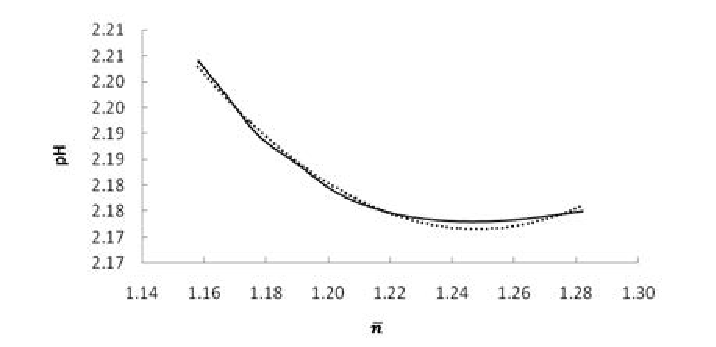
\includegraphics{figures/oxalic-acid-n-geq-1.15.pdf}
  \caption{乙二酸$\overline{n}\geq 1.15$数据段曲线及其拟合曲线 (实线--实际曲线, 虚线--拟合曲线) 乙二酸$\overline{n}\geq 1.15$数据段曲线及其拟合曲线 (实线--实际曲线, 虚线--拟合曲线) 乙二酸$\overline{n}\geq 1.15$数据段曲线及其拟合曲线 (实线--实际曲线, 虚线--拟合曲线)}
\end{figure}

在排版过程中我们会遇到多列子图的情况, 我们在文档类中已经引用了 \pckg{subcaption} 宏包, 并做好了子图的图序和图题的格式定制. 我们利用 \verb|subfigure| 环境来排版子图, 它的第一个可选参数 \verb|<outer-pos>| 表示子图整个盒子的垂直位置, 可选项为 ``c", ``t", ``b", ``T", ``B", 可以参考 \pckg{latex2e} 文档中关于 \verb|minipage| 环境及参数的介绍以及 \pckg{subcaption} 宏包文档的相关内容来明白这些参数以及其它可选参数的含义. \verb|subfigure| 环境的必选参数表示这张子图及图题所占的宽度, 它不会帮你缩放插图, 但会决定图题所占的宽度, 注意\verb|\linewidth| 表示去除边界之后的页面宽度, 一行之中所有子图的宽度之和不要超过这个宽度. 下面的例子中要注意仅在子图要换行的时候添加空行, 还要注意 \verb|\hfil| 宏保证了这些子图之间以及与页边的水平间距合适, 关于 \verb|\hfil| 宏可以参考\href{https://tex.stackexchange.com/a/528921/184559}{这个 TeX.SE 中的回答}.

\begin{figure}[htb]
  \hfil
  \begin{subfigure}[b]{0.4\linewidth}
    \centering
    
\includegraphics{tongji-name-bacholar.jpg}
    \caption{乙二酸$\overline{n}\geq 1.15$数据段曲线及其拟合曲线 (实线--实际曲线, 虚线--拟合曲线)}
  \end{subfigure}
  \hfil
  \begin{subfigure}[b]{0.4\linewidth}
    \centering
    
\includegraphics{tongji-name-bacholar.jpg}
    \caption{乙二酸$\overline{n}\geq 1.15$数据段曲线及其拟合曲线 (实线--实际曲线, 虚线--拟合曲线)}
  \end{subfigure}
  \hfil

  \hfil
  \begin{subfigure}[b]{0.4\linewidth}
    \centering
    
\includegraphics{tongji-name-bacholar.jpg}
    \caption{乙二酸$\overline{n}\geq 1.15$数据段曲线及其拟合曲线 (实线--实际曲线, 虚线--拟合曲线)}
  \end{subfigure}
  \hfil
  \begin{subfigure}[b]{0.4\linewidth}
    \centering
    
\includegraphics{tongji-name-bacholar.jpg}
    \caption{乙二酸$\overline{n}\geq 1.15$数据段曲线及其拟合曲线 (实线--实际曲线, 虚线--拟合曲线)}
  \end{subfigure}
  \hfil
  \caption{乙二酸$\overline{n}\geq 1.15$数据段曲线及其拟合曲线 (实线--实际曲线, 虚线--拟合曲线)}
\end{figure}

\zhlipsum[1]

\subsection{表格}

我们先来整理一下手册对插图的要求. 手册第十九页的撰写规范中提到:
\begin{quote}
  每个表格应有表序和表题, 表序和表题应写在表格上方正中, 表序后空一格书写表题. 表序, 表题采用宋体小5号. 表格允许下页接写, 表题可省略, 表头应重复写, 并在右上方注明 ``{\songti 续表XX}". 表格上下均应空一行.
\end{quote}
手册第五十一页及第五十二页的参考例文中提到:
\begin{quote}
  表格上下与正文之间各空一行;
  采用三线表, 两端与页面对齐;
  表中文字: 小五, 宋体 (英文 Times New Roman), 行距 18 磅, 段前 0 行, 段后 0 行.

  表序写在表题左方不加标点, 空一格写表题, 表题末尾不加标点, 表格逐章编序, 表序必须连续, 如表 4.4 表示第四章的第四个表. 表题: 小五, 宋体 (英文 Times New Roman), 居中置于表上方, 行距 18 磅, 段前 0 行, 段后 0 行.

  若表格分页, 则该表第 2 页的表题省略, 但表头应重写, 并在表右上方加注 ``续表 X.X";
  ``续表 X.X" 的格式: 小五, 宋体 (英文 Times New Roman), 行距 18 磅, 段前 0 行, 段后 0 行, 右空 2 格.
\end{quote}
